\documentclass[11pt]{article}
\usepackage[margin=1in]{geometry}
\usepackage{amsmath,amssymb,mathtools}
\usepackage{siunitx}
\usepackage{graphicx}
\usepackage[hidelinks]{hyperref}
\usepackage{float}
\usepackage{csvsimple}
\usepackage{booktabs}
\usepackage{caption}
\usepackage{pdfpages}
\usepackage{attachfile2}
\usepackage{pgfplots}
\pgfplotsset{compat=1.18}
\usepackage{pgfplotstable}

\title{PHY-202L — Lab 5: Solenoid Field}
\author{Jake Killian}
\date{September 29, 2025}

\begin{document}
\maketitle

\section{Abstract}
The goal of this lab is for students to become familiar with the on-axis magnetic field of a solenoid.
Students will do this by measuring the on-axis magnetic field of a solenoid at various distances from the center of the solenoid.
Students will then compare their measurements to theoretical models from both the Laboratory Manual and the textbook.

\section{Theory}
Loop model:
\[
B_z(z) = \frac{\mu_0 N I R^2}{2\,(z^2 + R^2)^{3/2}}.
\]
Finite solenoid:
\[
B_z(z)=\frac{\mu_0 n I}{2}\!\left(
\frac{z+\tfrac{L}{2}}{\sqrt{(z+\tfrac{L}{2})^2+R^2}}
-\frac{z-\tfrac{L}{2}}{\sqrt{(z-\tfrac{L}{2})^2+R^2}}
\right),\quad n=\frac{N}{L}.
\]

\section{Procedure}
\begin{enumerate}
    \item Set up the sensor and solenoid as stated in the Laboratory Manual
    \item Set the sensor to the correct range and zero
    \item Turn on the power supply and set it to 0.3 A
    \item Measure the magnetic field at 1 cm intervals from the center of the solenoid
    \item Record the data in a table
    \item When the measurements begin to plateau: switch power supply off, set new sensor range, re-zero sensor, resume measurements until data plateaus
    \item Switch power supply off
    \item Record the length, radius, and number of turns of the solenoid
\end{enumerate}

\section{Raw Data}
\begin{table}[H]
    \centering
    \caption{Raw data imported from CSV file}
    \label{tab:rawcsv}
    \csvautotabular{\detokenize{../data/raw/Lab_5.csv}}
\end{table}

\section{Analysis and Results}
Figure~\ref{fig:b_z-vs-z} shows the magnetic field as a function of distance from the center of the solenoid.
The figure shows side-by-side comparisons of the experimental data with the two theoretical models.
All three curves show a good agreement towards the latter end of the data set, where cubic falloff is expected.
However, there are some discrepancies between the experimental data and the theoretical models near the center of the solenoid.
Possible reasons for these discrepancies are discussed in the Error Analysis section.
\footnote{A full step-by-step analysis (data wrangling, calculations, visualizations) of the data is included in the appendix as a Jupyter Notebook.}

A traditional trendline analysis was not performed, as the data is not expected to follow any common mathematical function.
Instead, the experimental data was compared directly to the two theoretical models.
The closest agreement between the experimental data would be a cubic falloff, which is expected beyond the fringe fields of the solenoid.
However, fringe fields are expected to be present in the data set, as the data set includes measurements taken near the center of the solenoid.

Overall, the experimental data shows a general shape-wise agreement with both theoretical models.

\begin{figure}[H]
    \centering
    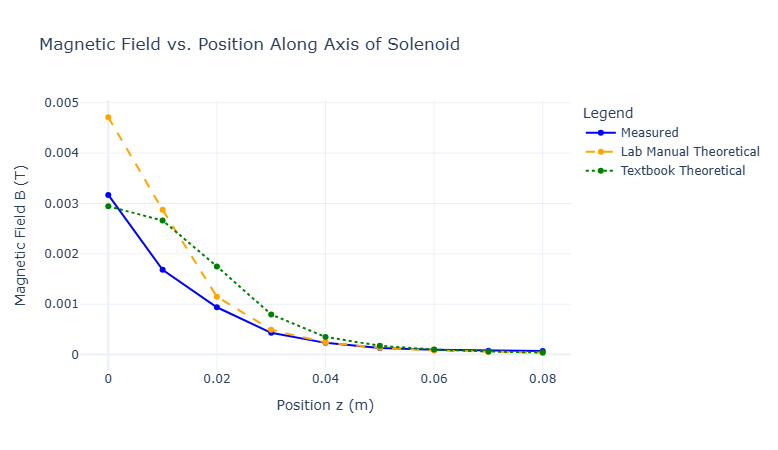
\includegraphics[width=0.8\linewidth]{../notebooks/figures/fig1.png}
    \caption{Magnetic field measurements and theoretical models}
    \label{fig:b_z-vs-z}
\end{figure}

\section{Error Analysis}
Figure~\ref{fig:percent-error} shows the percent error between the experimental data and the two theoretical models.
As shown in the figure, both the textboook and Lab Manual models show similar percent errors throughout the data set.
In both models, the percent error has a local maximum near the center of the solenoid.
Both models also show a generally decreasing percent error as the distance from the center of the solenoid increases, with the exception of the final data points.
A significant difference between the two models is that the Lab Manual model shows a slightly lower percent error throughout the experimental data set.
Interestingly, the textbook model shows a slightly lower percent error at the initial data point of $z=\SI{0}{\meter}$.
Both models show an extremely high percent error at the final data points, which goes against their previous trend of generally becoming more accurate as distance increases.
This is likely due to the magnetic field approaching the floor of the sensor's range, which would cause the sensor to be both less accurate and possibly even become saturated.
Upon data analysis, it is recommended that at a minimum the final data point be discarded, as data at this point is likely unreliable.
Further investigation and testing should be done to determine sensor accuracy limits at low magnetic field strengths.

Figure~\ref{fig:b_z-vs-z} indicates that another possible error could be due to the solenoid not being perfectly aligned with the sensor at $z=\SI{0}{\meter}$.
This would reduce the accuracy of the measurements systematically, especially near the center of the solenoid.
Further analysis should be done to determine if offsetting the sensor position addresses this hypothesis.

\subsection*{Additional possible sources of error}
\begin{itemize}
    \item The current through the solenoid may not be perfectly constant at $\SI{0.3}{\ampere}$
    \item The sensor may not be perfectly calibrated
    \item There may be interference from external magnetic fields
\end{itemize}

\begin{figure}[H]
    \centering
    \begin{tikzpicture}
    \begin{axis}[
        width=0.8\linewidth,
        xlabel={$z$ (meter)},
        ylabel={Percent Error (\%)},
        grid=both,
        legend pos=north east,
    ]

    % Textbook % Error
    \addplot table[
        col sep=comma,
        x={z (m)},
        y={Relative Error (Textbook)}
    ]{../data/processed/Lab_5_clean.csv};
    \addlegendentry{Textbook Model}

    % Lab Manual % Error
    \addplot table[
        col sep=comma,
        x={z (m)},
        y={Relative Error (Lab Manual)}
    ]{../data/processed/Lab_5_clean.csv};
    \addlegendentry{Lab Manual Model}
\end{axis}
\end{tikzpicture}
\caption{Percent error between experimental data and theoretical models}
\label{fig:percent-error}
\end{figure}

\section{Conclusion}
Placeholder text
In this lab, the on-axis magnetic field of a solenoid was measured and compared to two theoretical models.
The experimental data showed a general shape-wise agreement with both theoretical models.
Both models showed a similar percent error trend, with the Lab Manual model showing a slightly lower percent error overall.
However, both models showed a significant increase in percent error at the final data points, likely due to sensor limitations at low magnetic field strengths.
Possible sources of error were discussed, most notably with the potential misalignment of the solenoid and sensor.
\footnote{An initial analysis showed a possible offset of 5.5 mm might minimize the global percent error. However, this was not confirmed as developing and explaining the math behind this was deemed out of scope for this lab. Further investigation is recommended.}
Further investigation and testing is recommended to address the sources of error discussed in the Error Analysis section.
Additionally, further analysis could be done to minimize the percent error by optimizing the sensor position.
Overall, the lab should be considered a success, as the theoretical models were proven with relatively low error rates.

\appendix
\section{Full Jupyter Notebook}
\includepdf[pages=-]{../notebooks/Lab_5.pdf}
\bigskip
\noindent The original notebook file is attached here: \attachfile{../notebooks/Lab_5.ipynb}

\end{document}
